\documentclass{article}
\usepackage[margin=1.0in]{geometry}
\usepackage[usenames, dvipsnames]{color}
\usepackage{longtable}
\usepackage[flushleft]{threeparttable}
\usepackage[justification=centering]{caption}
\usepackage{tikz}
\usepackage{pgfplots}
\usepackage{amsthm}
\usepackage{amsmath}
\usepackage{amssymb}
\usepackage[sc]{mathpazo}
\usepackage{microtype}
\usepackage[english]{babel}
\usepackage{titlesec}
\usepackage{physics}
\usepackage{float}
\usepackage{fancybox,framed}
\usepackage{graphicx}
\usepackage{caption}
\usepackage{subcaption}
\usepackage{cprotect}
\titleformat{\section}[block]{\large\scshape}{\thesection.}{1em}{} 
\titleformat{\subsection}[block]{\large}{\thesubsection.}{1em}{}

\newcommand\tab[1][1cm]{\hspace*{#1}}
\renewcommand\op[1]{\hat{#1}}
\title{PHYS 512 - Assignment 1}
\author{André Vallières (260742187)}
\date{\today}

\begin{document}
\maketitle

\section*{Problem 1}
\begin{itemize}
    \item[a) ] First, we let
    \begin{align*}
        f'_1 (x) &= \frac{f(x + \delta) - f(x - \delta)}{2\delta} \\
        f'_2 (x) &= \frac{f(x + 2\delta) - f(x - 2\delta)}{4\delta}
    \end{align*}
    
    Ignoring finite machine precision for now, we have, in general
    \begin{align*}
        f(x + \alpha \delta) = f(x) = \alpha \delta f'(x) + \frac{(\alpha \delta)^2}{2} f''(x) + \frac{(\alpha \delta)^3}{6} f'''(x) + ...
    \end{align*}
    
    Hence, 
    \begin{align*}
        f'_1 (x) &= \frac{(f(x) + \delta f'(x) + \delta^2 f''(x) / 2 + \delta^3 f'''(x) / 6 + ...) - (f(x) - \delta f'(x) + \delta^2 f''(x) / 2 - \delta^3 f'''(x) / 6 + ...) \Big]}{2\delta} \\
        &= f'(x) + \frac{\delta^2}{6} f'''(x) + ...
    \end{align*}
    
    and
    \begin{align*}
        f'_2 (x) &= \frac{(f(x) + 2\delta f'(x) + 2 \delta^2 f''(x) + 4 \delta^3 f'''(x) / 3 + ...) - (f(x) - 2 \delta f'(x) + 2 \delta^2 f''(x) - 4 \delta^3 f'''(x) / 3 + ...) \Big]}{4\delta} \\
        &= f'(x) + 4 \frac{\delta^2}{6} f'''(x) + ...
    \end{align*}
    
    Using these two equations, we get
    \begin{align}
        \label{eq:sol-1a}
        f'_{\text{approx}}(x) = \frac{f'_2(x) - 4f'_1(x)}{-3} + \mathcal{O}(f^{(5)}(x))
    \end{align}
    
    which eliminates the third-order term.
    
    \item[b)] To find $\delta$ in terms of the machine precision ($\varepsilon$) and various properties of the function, we need to account for finite machine precision in the Taylor series and include the fifth-order term.
    
    Expanding from our previous equations, we have
    \begin{align*}
        f'_1(x) &= f'(x) + \frac{\delta^2}{6} f'''(x) + \frac{\delta^4}{120} f^{(5)}(x) + \frac{g_1 \varepsilon f(x) }{2 \delta} + ...\\
        f'_2 (x) &= f'(x) + 4 \frac{\delta^2}{6} f'''(x) + \frac{\delta^4}{15} f^{(5)}(x) + \frac{g_2 \varepsilon f(x) }{4 \delta} + ...
    \end{align*}
    
    Thus, (\ref{eq:sol-1a}) becomes
    \begin{align}
        f'_{\text{approx}}(x) = f'(x) + \frac{\delta^4}{15}f^{(5)}(x) + \frac{\varepsilon}{\delta} \Big( \frac{g_2}{4} - 2 g_1 \Big) f(x) + ...
    \end{align}
    
    If we let
    \begin{align*}
        \Delta \equiv \frac{\delta^4}{15}f^{(5)}(x) + \frac{\varepsilon}{\delta} \Big( \frac{g_2}{4} - 2 g_1 \Big) f(x) = \frac{\delta^4}{15}f^{(5)}(x) + \frac{\varepsilon}{\delta} g f(x)
    \end{align*}
    
    Then the error is minimized if
    \begin{align*}
        \frac{d\Delta}{d\delta} &= \frac{4 \delta^3}{15}f^{(5)}(x) - \frac{g \varepsilon}{\delta^2} f(x) = 0\\
        &\Rightarrow \delta^5 = \frac{15 g \varepsilon}{4} \frac{f(x)}{f^{(5)}(x)} \sim \frac{15 \varepsilon}{4} \frac{f(x)}{f^{(5)}(x)}\\
        &\Rightarrow \delta = \Big( \frac{15 \varepsilon}{4} \frac{f(x)}{f^{(5)}(x)} \Big)^{1/5}
    \end{align*}
    
    Given $\varepsilon = 10^{-16}$, we have that the error is minimized for
    \begin{equation*}
        \delta \approx 
        \begin{cases}
        8 \times 10^{-4} & \text{ for } f(x) = \exp(x)\\
        8 \times 10^{-2} & \text{ for } f(x) = \exp(0.01x)
        \end{cases}
    \end{equation*}
    
    The code to verify these estimates is in \verb|prob1_b.py|. The results are 
    \begin{equation*}
        \delta \approx 
        \begin{cases}
        8 \times 10^{-4} & \text{ for } f(x) = \exp(x)\\
        1 \times 10^{-2} & \text{ for } f(x) = \exp(0.01x)
        \end{cases}
    \end{equation*}
    
    Of course, the estimates are not exact, but at least we see a factor near $1/100$ as expected from the rough calculations.
\end{itemize}

\newpage
\section*{Problem 2}
Using Hermite polynomials for interpolating due to the features at low temperature, we arrive at a pretty accurate model. The code is in \verb|prob2.py|, and performs two tasks: 1) Interpolate with odd points 2) Compute RMS error using even points. Plotting the real and interpolated data simply shows no visible difference, as seen in Figure 1. The RMS error, however, computed as \verb|np.std(true - estimate)|, gives \textbf{0.032102}. The reason for using different points for interpolating and computing the error is to minimize bias. Indeed, using all points simply yields a null RMS error for points in the dataset, but the model would obviously not be free of discepancies from reality.

\begin{figure}[h]
    \centering
    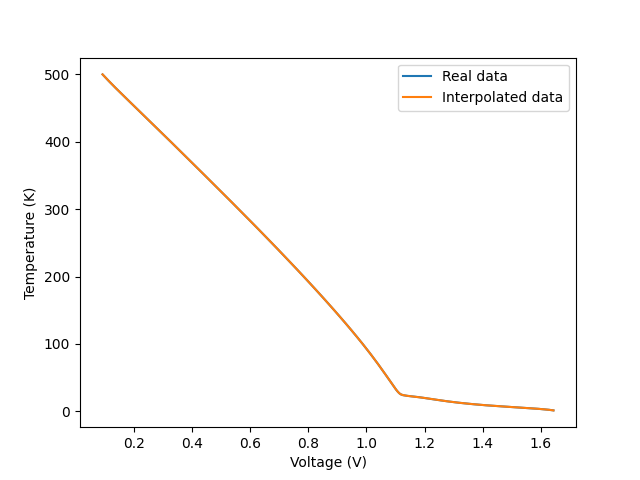
\includegraphics[scale=0.8]{images/prob2_lakeshore_interp}
    \caption{Real and interpolated data for DT-670 silicon diode using Hermite polynomial interpolation.}
\end{figure}

\newpage
\section*{Problem 3}
The code for polynomial, cubic spline, and rational interpolation is in \verb|prob3.py|. To evaluate them on the same ground, 4 points are used for interpolation. The first function to interpolate is $cos(x)$ in the range $[-\pi/2,\pi/2]$. The results are shown in Figure 2.
\begin{figure}[h!]
\centering
\begin{subfigure}{.5\textwidth}
  \centering
  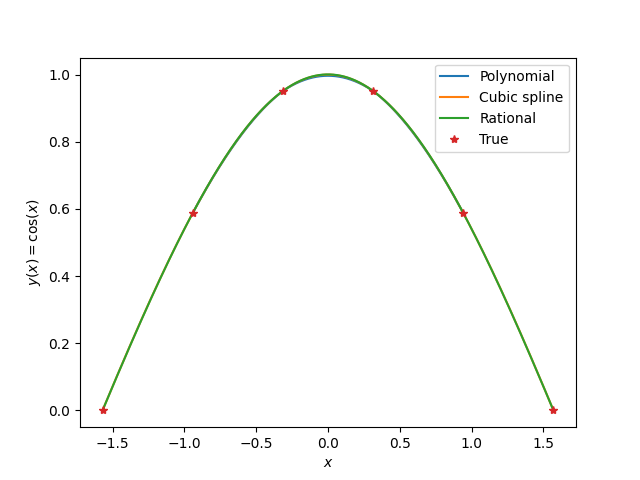
\includegraphics[width=\linewidth]{images/prob3_cos_func.png}
  \caption{}
\end{subfigure}%
\begin{subfigure}{.5\textwidth}
  \centering
  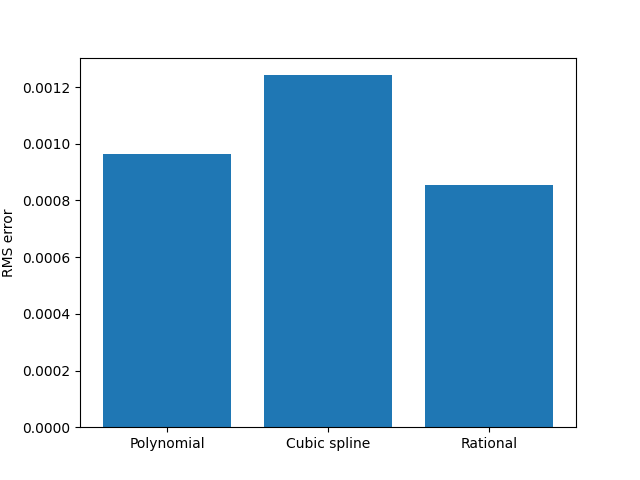
\includegraphics[width=\linewidth]{images/prob3_cos_errs.png}
  \caption{}
\end{subfigure}
\caption{Cosine interpolation results for cubic polynomial, cubic spline, and rational interpolation with $n=2, m=3$. (a) Interpolation of $cos(x)$ in the range $[-\pi/2, \pi/2]$ showing great fit. (b) RMS error for all three interpolation methods. Rational interpolation shows best fit.}
\label{fig:cos_results}
\end{figure}

The second function to interpolate is a Lorentzian, so $1/(1+x^2)$ in the range $[-1, 1]$. We expect rational interpolation to perform best since a Lorentzian is a polynomial function. Running interpolation with the same parameters as before yields results shown in Figure 3.
\begin{figure}[h!]
\centering
\begin{subfigure}{.5\textwidth}
  \centering
  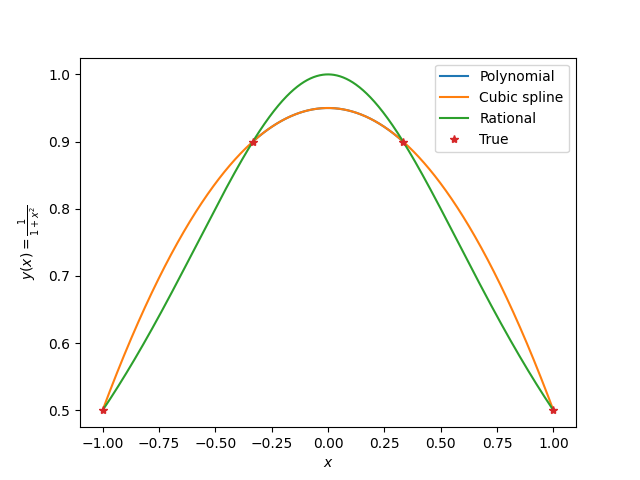
\includegraphics[width=\linewidth]{images/prob3_lorentzian_func_4points.png}
  \caption{}
\end{subfigure}%
\begin{subfigure}{.5\textwidth}
  \centering
  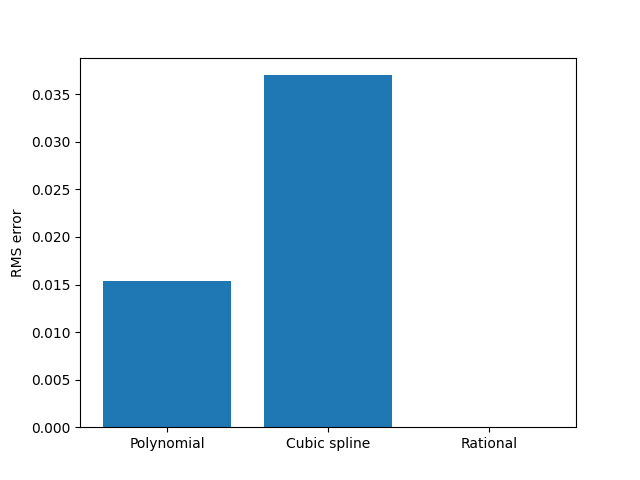
\includegraphics[width=\linewidth]{images/prob3_lorentzian_errs_4points.png}
  \caption{}
\end{subfigure}
\caption{Lorentzian interpolation results for cubic polynomial, cubic spline, and rational interpolation with $n=2, m=3$. (a) Interpolation of $1/(1+x^2)$ in the range $[-1, 1]$ showing perfect fit for rational interpolation. (b) RMS error for all three interpolation methods. Rational interpolation again shows best fit with a null RMS error.}
\label{fig:lorentzian_4points_results}
\end{figure}

Now, if we were to increase the number of points (to 8, for example), we would expect similar results. Polynomial and cubic spline interpolation may perform better, but rational interpolation should still have perfect fit. However, this is not what happens. In fact, doing interpolation with $n=4, m=5$ yields very poor results for rational interpolation as shown in Figure 4.
\begin{figure}[h!]
\centering
\begin{subfigure}{.5\textwidth}
  \centering
  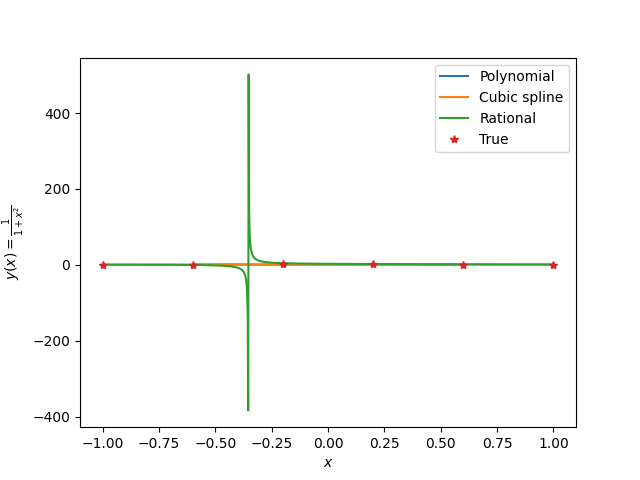
\includegraphics[width=\linewidth]{images/prob3_lorentzian_func.png}
  \caption{}
\end{subfigure}%
\begin{subfigure}{.5\textwidth}
  \centering
  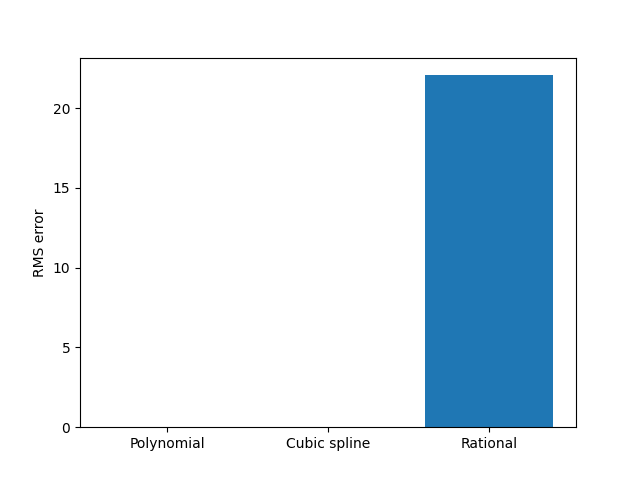
\includegraphics[width=\linewidth]{images/prob3_lorentzian_errs.png}
  \caption{}
\end{subfigure}
\caption{Lorentzian interpolation results for cubic polynomial, cubic spline, and rational interpolation with $n=4, m=5$. (a) Interpolation of $1/(1+x^2)$ in the range $[-1, 1]$ showing extremely poor fit for rational interpolation. (b) RMS error for all three interpolation methods. Rational interpolation is so high polynomial and cubic spline interpolation errors show as 0 (although there are around $0.00118$ and $0.000675$, respectively).}
\label{fig:lorentzian_4points_results}
\end{figure}

By simply changing \verb|np.linalg.inv| to \verb|np.linalg.pinv| in the \verb|rat_fit| function solves the issue, as shown in Figure 5. The change makes sure the fitting step can deal with singular matrix inversion.
\begin{figure}[h!]
\centering
\begin{subfigure}{.5\textwidth}
  \centering
  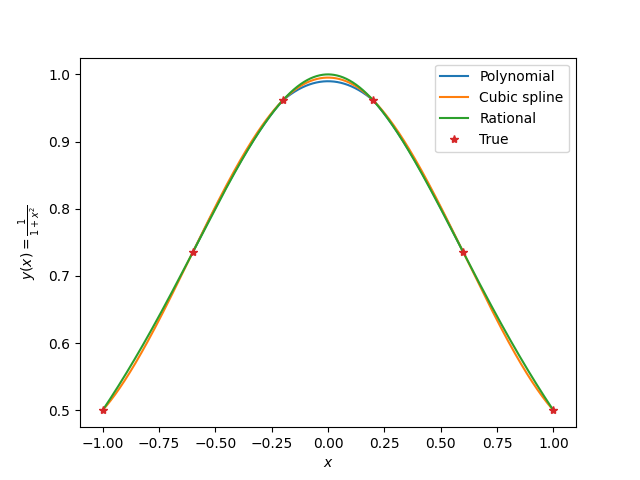
\includegraphics[width=\linewidth]{images/prob3_lorentzian_func_pinv.png}
  \caption{}
\end{subfigure}%
\begin{subfigure}{.5\textwidth}
  \centering
  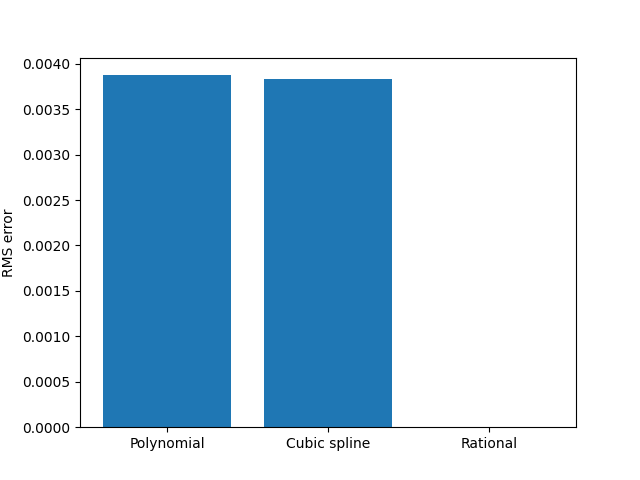
\includegraphics[width=\linewidth]{images/prob3_lorentzian_errs_pinv.png}
  \caption{}
\end{subfigure}
\cprotect\caption{Lorentzian interpolation results for cubic polynomial, cubic spline, and rational interpolation with $n=4, m=5$ using \verb|np.linalg.pinv|. (a) Interpolation of $1/(1+x^2)$ in the range $[-1, 1]$ showing back perfect fit for rational interpolation. (b) RMS error for all three interpolation methods. Rational interpolation is so high polynomial and cubic spline interpolation errors show as 0 (although there are around $0.00118$ and $0.000675$, respectively.}
\label{fig:lorentzian_pinv_results}
\end{figure}

Investigating a bit on why it failed miserably before, as shown in Figure 4, we look at the \verb|rat_fit| function. We notice that the determinant of the matrix that we build is really close to zero, but not exactly due to numerical imprecision. For example, with $n=3, m = 4$, the determinant is of the order of $4.3 \times 10^{-18}$. This is effectively zero and no real inverse can be computed. This is why we needed \verb|np.linalg.pinv| to compute the pseudo-inverse. However, practically, the determinant is not exactly zero thus the inversion process carries on but the calculated matrix inverse will have unusually large numbers due to the $1/\text{det}(M)$ factor. In fact, this could turn practically zero values (i.e., really near zero, but not exactly due to numerical imprecision) into appreciable values, which would screw up the fitting process. If we look at the entries in $p$ and $q$, some entries are greater than 1, which should not happen. As we increase $n$ and $m$, those values increase to higher numbers which cause the poor fitting. For example, in Figure 6, the top portion corresponds to calculations with \verb|np.linalg.inv| and the bottom with \verb|np.linalg.pinv|. Notice the huge difference of magnitude between the entries of $p$ and $q$.
\begin{figure}[h]
    \centering
    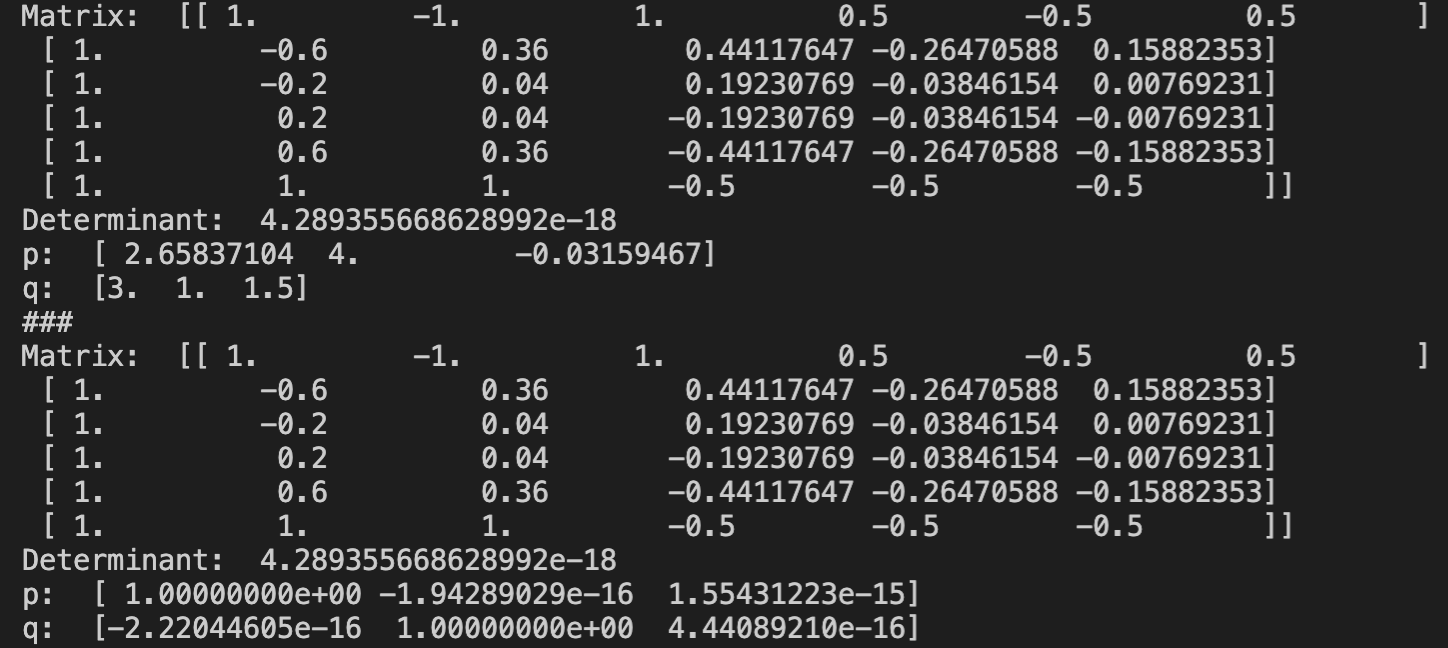
\includegraphics[scale=0.5]{images/prob3_pq_explanation.png}
    \cprotect\caption{Top: Rational function fitting using \verb|np.linalg.inv|. Bottom: Rational function fitting using \verb|np.linalg.pinv|. Notice the huge difference in magnitudes of the entries of $p$ and $q$ for those two approaches.}
\end{figure}

\newpage
\section*{Problem 4}
From Griffiths's solutions, the electric field from an infinitesimally thin spherical shell of charge with radius R is given by
\begin{equation}
    E = \frac{\sigma}{4 \pi \epsilon_0} \int_0^\pi \frac{(z - R \cos \theta)(2 \pi R \sin \theta)}{z^2 + R^2 - 2 z R \cos \theta}^{3/2} R d\theta
\end{equation}

where $z$ is the distance from the center. In cgs units, we can simply discard the $4 \pi \epsilon_0$ factor, and for the purpose of this demonstration, we let $\sigma = 1$.

The integrator I've decided to use is the variable step size integrator shown in class due to its ability to find sharp features, such as the electric field at the spherical shell boundary. Running through the integration with different $z$, we notice a problem with the singularity at $z = R$. This is due to the discontinuity of the electric field at the boundary which means the integrand's denominator is 0 during the integration. To solve this issue, I first simply ignored integration that returned NaN, but that would give a discontinuity in the electric field versus distance plot. Hence, I decided to instead change the electric field formula to
\begin{equation}
    E = \int_0^\pi \frac{(z - R \cos \theta)(2 \pi R \sin \theta)}{z^2 + R^2 - 2 z R \cos \theta + \epsilon}^{3/2} R d\theta
\end{equation}

where I've set $\epsilon = 10^{-16}$. Doing so, the integration at $z = R$ is correctly handled and the results are shown in Figure 7. Interestingly, no such trick is needed with the \verb|scipy.integrate.quad| function, which correctly handles singularities.
\begin{figure}[h]
    \centering
    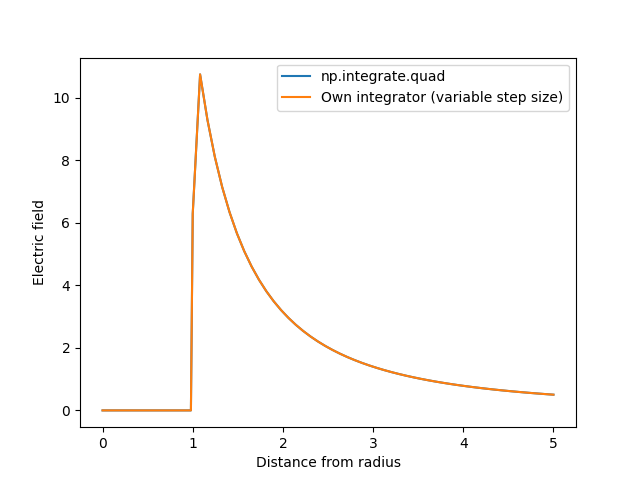
\includegraphics[scale=0.8]{images/prob4_electric_field.png}
    \cprotect\caption{Electric field as a function of the distance from the radius, $R$, which is set to $1$. This is found by integration following (4). The RMS difference between results found with \verb|scipy.integrate.quad| or \verb|my_integrate| is around $9.3 \times 10^{-5}$.}
\end{figure}

\end{document}